\documentclass[convert={density=300,size=1080x800,outext=.png}]{standalone}
\usepackage{tkz-graph}
\usetikzlibrary{arrows,positioning,shapes,shapes.multipart,patterns,mindmap,shadows}
\usepackage{xcolor}
\usepackage{helvet}
\renewcommand{\familydefault}{\sfdefault}


\begin{document}

\footnotesize
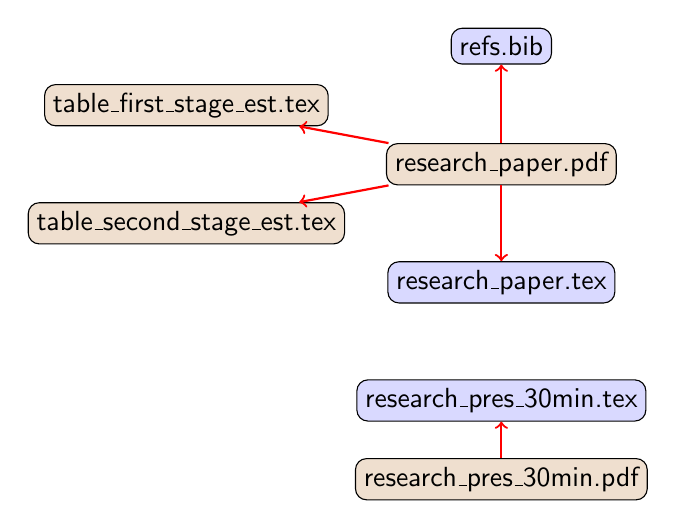
\begin{tikzpicture}[every node/.style={
    rectangle,
    rounded corners,
    inner sep=3pt,
    draw,
    fill=brown!25
}]
    \node (research_paper_tex) [fill=blue!15, shift={(19, 0.5)}]
    {
        research\_paper.tex
    };

    \node (research_paper_pdf) [shift={(19, 2)}]
    {
        research\_paper.pdf
    };


    \node (research_pres_30min_tex) [fill=blue!15, shift={(19, -1)}]
    {
        research\_pres\_30min.tex
    };

    \node (research_pres_30min_pdf) [shift={(19, -2)}]
    {
        research\_pres\_30min.pdf
    };

    \node (refs_bib) [fill=blue!15, shift={(19, 3.5)}]
    {
        refs.bib
    };

    \node (table_first_stage_est_tex) [shift={(15, 2.75)}]
    {
        table\_first\_stage\_est.tex
    };

    \node (table_second_stage_est_tex) [shift={(15, 1.25)}]
    {
        table\_second\_stage\_est.tex
    };




    \draw[->, red, thick] (research_paper_pdf) to (research_paper_tex);
    \draw[->, red, thick] (research_pres_30min_pdf) to (research_pres_30min_tex);


    \draw[->, red, thick] (research_paper_pdf) to (table_first_stage_est_tex);
    \draw[->, red, thick] (research_paper_pdf) to (table_second_stage_est_tex);
    \draw[->, red, thick] (research_paper_pdf) to (refs_bib);
\end{tikzpicture}

\end{document}
